% alganal.tex
% A Practical Introduction to Data Structures and Algorithm Analysis
% 3rd Edition: Shared between C++ and Java versions

\chapter{Algorithm Analysis}
\label{AlgAnal}
\def\CHHEAD{Chap.\ \thechapter\ Algorithm Analysis}    % Head title -- even pages

% ``Questions about a theory which do not affect its ability to
% predict experimental results correctly seem to me quibbles about
% words, ... and I am quite content to leave such questions to those
% who derive some satisfaction from them.'' -- John C. Slater

\index{algorithm analysis|(}
How long will it take to process the company payroll once we complete
our planned merger?
Should I buy a new payroll program from vendor X or vendor Y?
If a particular program is slow, is it badly implemented or is it
solving a hard problem?
Questions like these ask us to consider the difficulty of a problem,
or the relative efficiency of two or more approaches to solving a
problem.

This chapter introduces the motivation, basic notation, and
fundamental techniques of algorithm analysis.
We focus on a methodology known as
\defit{asymptotic algorithm analysis}, or simply
\defit{asymptotic analysis}.\index{algorithm analysis!asymptotic}
Asymptotic analysis attempts to estimate the resource
consumption of an algorithm.\index{estimation}
It~allows us to compare the relative costs of two or more
algorithms for solving the same problem.
Asymptotic analysis also gives algorithm designers a tool for
estimating whether a proposed solution is likely to meet the resource
constraints for a problem before they implement an actual
program.\index{estimation}\index{resource constraints}
After reading this chapter, you should understand

\begin{itemize}
\item
the concept of a growth rate\index{growth rate},
the rate at which the cost of an algorithm grows
as the size of its input grows;

\item
\index{upper bound}
\index{lower bound}
the concept of upper and lower bounds for a
growth rate, and how to estimate these bounds for a simple program,
algorithm, or problem; and\index{estimation}

\item
the difference between the cost of an algorithm
(or program) and the cost of a problem.
\index{problem!analysis of}
\end{itemize}

\noindent The chapter concludes with a brief discussion of the practical
difficulties encountered when empirically
measuring\index{algorithm analysis!empirical comparison} the cost of a
program, and some principles for code tuning
to improve program efficiency.\index{code tuning}

\section{Introduction}
\label{AnalIntro}

\index{algorithm analysis!empirical comparison|(}
How do you compare two algorithms for solving some problem in terms
of efficiency?
We could implement both algorithms as computer programs and then
run them on a suitable range of inputs, measuring how much of the
resources in question each program uses.
This approach is often unsatisfactory for four reasons.
First, there is the effort involved in programming and testing two
algorithms when at best you want to keep only one.
Second, when empirically comparing two algorithms there
is always the chance that one of the programs was ``better written''
than the other, and therefor the relative qualities of the underlying
algorithms are not truly represented by their implementations.
This can easily occur when the programmer has a bias
regarding the algorithms.
Third, the choice of empirical test cases might unfairly favor one
algorithm.
Fourth, you could find that even the better of the two algorithms does
not fall within your resource budget\index{resource constraints}.
In that case you must begin the entire process again with yet another
program implementing a new algorithm.
But, how would you know if any algorithm can meet the resource budget?
Perhaps the problem is simply too difficult for any implementation to
be within budget.
\index{algorithm analysis!empirical comparison|)}

These problems can often be avoided by using 
asymptotic analysis.\index{algorithm analysis!asymptotic}
Asymptotic analysis measures the efficiency of an algorithm, or its
implementation as a program, as the input size becomes large.
It is actually an estimating technique\index{estimation}
and does not tell us anything about the relative merits of two
programs where one is always ``slightly faster'' than the other.
However, asymptotic analysis has proved useful
to computer scientists who must determine if a particular algorithm
is worth considering for implementation.

The critical resource for a program is most often its running
time.
However, you cannot pay attention to running time alone.
You must also be concerned with other factors such as the space
required to run the program (both main memory and disk space).
Typically you will analyze the \emph{time} required for an
\emph{algorithm} (or the instantiation of an algorithm in the form
of a program), and the \emph{space} required for a
\emph{data structure}. 
\index{algorithm analysis!space requirements}

\index{program!running time|(}
Many factors affect the running time of a program.
Some relate to the environment in which the program
is compiled and run.
Such factors include the speed of the computer's CPU, bus, and
peripheral hardware.
Competition with other users for the computer's (or the network's)
resources can make a program slow to a crawl.
The programming language and the quality of code generated by a
particular compiler can have a significant
effect.\index{compiler!efficiency}
The ``coding efficiency''\index{code tuning} of the programmer
who converts the algorithm to a program can have a tremendous impact
as well.

If you need to get a program working within time and space
constraints on a particular computer, all of these factors can be
relevant.
Yet, none of these factors address the differences between
two algorithms or data structures.
To be fair, programs derived from two algorithms for solving the same
problem should both be compiled with the same compiler
and run on the same computer under the same conditions.
As much as possible, the same amount of care should be taken in
the programming effort devoted to each program to make the
implementations ``equally efficient.''\index{code tuning}
In this sense, all of the factors mentioned above should cancel
out of the comparison because they apply to both algorithms equally.

\index{algorithm analysis!running time measures}
If you truly wish to understand the running time of an algorithm,
there are other factors that are more appropriate to consider than
machine speed, programming language, compiler, and so
forth.
Ideally we would measure the running time of the algorithm under
standard benchmark conditions.
However, we have no way to calculate the running time reliably other
than to run an implementation of the algorithm on some computer.
The only alternative is to use some other measure as a surrogate for
running time.

Of primary consideration when estimating an algorithm's performance
is the number of\index{estimation}
\defit{basic operations}\index{basic operation} required by
the algorithm to process an input of a certain
\defit{size}.\index{input size}
The terms ``basic operations'' and ``size'' are both
rather vague and depend on the algorithm being analyzed.
Size is often the number of inputs processed.
For example, when comparing sorting algorithms\index{sorting},
the size of the problem is typically measured by the number of
records to be sorted. 
A basic operation must have the property that its time to
complete does not depend on the particular values of its operands.
Adding or comparing two integer variables are examples of basic
operations in most programming languages.
Summing the contents of an array containing \(n\)~integers is not,
because the cost depends on the value of \(n\) (i.e., the size of the
input).
\index{algorithm analysis!running time measures}
\index{program!running time|)}

\begin{example}
\label{SeqMax}
\index{search!sequential|(}
Consider a simple algorithm to solve the problem of finding the
largest value in an array of \(n\) integers.
The algorithm looks at each integer in turn, saving the position of
the largest value seen so far.
This algorithm is called the \emph{largest-value sequential search}
and is illustrated by the following function:

\xprogexamp{largest.book}

\noindent Here, the size of the problem is \Cref{A.length},
the number of integers stored in array \Cref{A}.
The basic operation\index{basic operation}
is to compare an integer's value to that of the
largest value seen so far.
It is reasonable to assume that it takes a fixed amount of time to do
one such comparison, regardless of the value of the two
integers or their positions in the array.

Because the most important factor affecting running time is normally
size of the input, for a given input size \(n\) we often express the
time~{\bf T} to  run the algorithm as a function of~\(n\), written
as~\Tn.\index{running-time equation}
We will always assume \Tn\ is a non-negative value.

Let us call~\(c\) the amount of time required to compare two integers
in function \Cref{largest}.
We do not care right now what the precise value of~\(c\) might be.
Nor are we concerned with the time required to increment
variable~\(i\) because this must be done for each value in the array,
or the time for the actual assignment when a larger value is found,
or the little bit of extra time taken to initialize \Cref{currlarge}.
We just want a reasonable approximation for the time taken to execute
the algorithm.
The total time to run \Cref{largest} is therefore approximately \cn,
because we must make \(n\) comparisons, with each comparison
costing~\(c\) time.
We say that function \Cref{largest}
(and by extension ,the largest-value sequential search algorithm for
any typical implementation) has a running time expressed
by the equation
\[\Tn = \cn.\]
\noindent This equation describes the
growth rate\index{growth rate} for the
running time of the largest-value sequential search
algorithm.\index{search!sequential|)}
\end{example}

\begin{example}

The\index{growth rate!constant}
running time of a statement that assigns the first value of an
integer array to a variable is simply the time required to copy the
value of the first array value.
We can assume this assignment takes a constant amount of time
regardless of the value.
Let us call \(c_1\) the amount of time necessary to copy an integer.
No matter how large the array on a typical computer (given reasonable
conditions for memory and array size), the time to copy the value from
the first position of the array is always \(c_1\).
Thus, the equation for this algorithm is simply
\[\Tn = c_1,\]
indicating that the size of the input \(n\) has no effect on
the running time.
This is called a \defit{constant} running time.
\index{growth rate!constant}
\end{example}

\begin{example}
Consider the following code:

\xprogexamp{c3p1.book}

What is the running time for this code fragment?
Clearly it takes longer to run when \(n\) is larger.
The basic operation\index{basic operation} in this example is the
increment operation for variable \emph{sum}.
We can assume that incrementing takes constant time;
call this time \(c_2\).
(We can ignore the time required to initialize \emph{sum}, and to
increment the loop counters \(i\) and \(j\).
In practice, these costs can safely be bundled into time \(c_2\).)
The total number of increment operations is \(n^2\).
Thus, we say that the running time is
\(\Tn = c_2 n^2.\)
\end{example}

\index{growth rate|(}

\begin{figure}
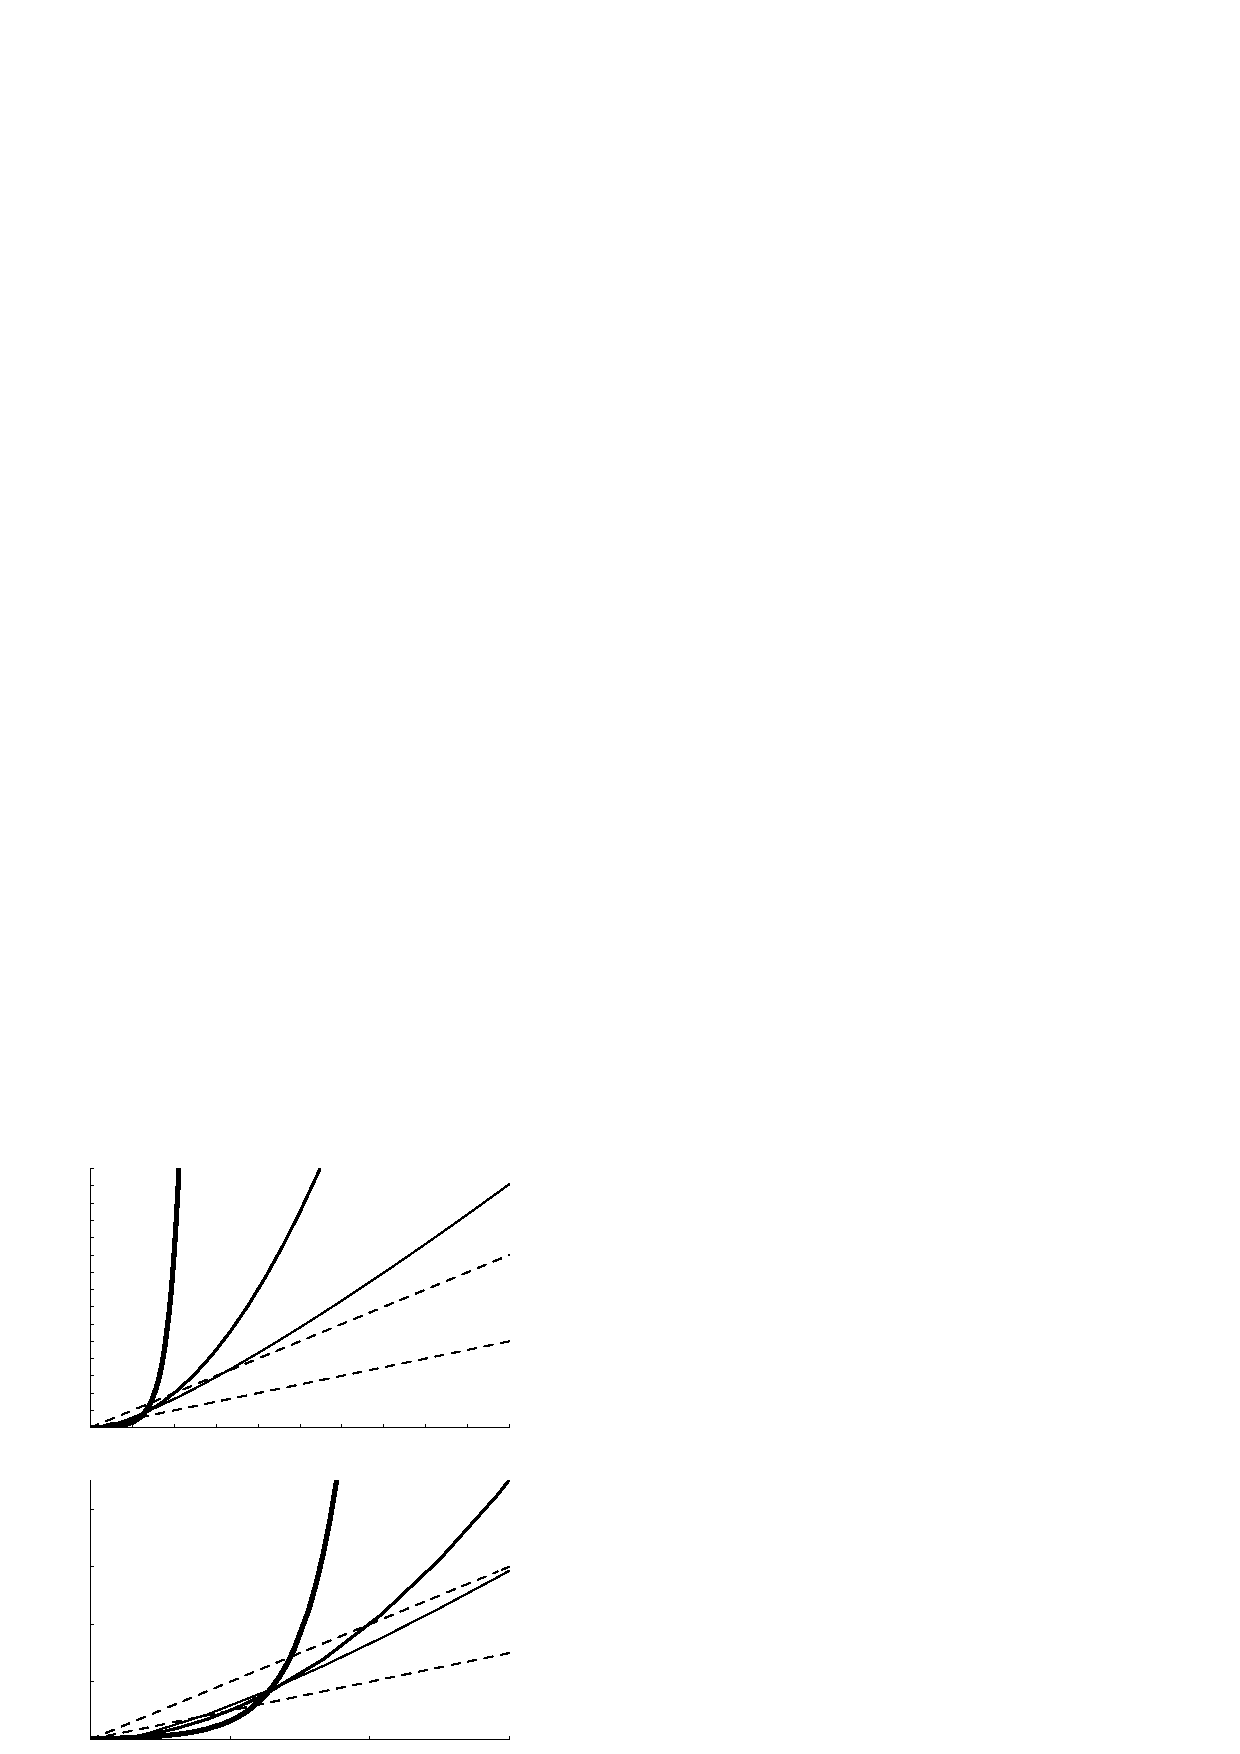
\includegraphics[viewport= 122 200 300 625]{../figs/plot.pdf}
\capt{4.5in}{The growth rates for five equations}
{Two views of a graph illustrating the growth rates for
six equations.
The bottom view shows in detail the lower-left portion
of the top view.
The horizontal axis represents input size.
The vertical axis can represent time, space, or any other measure of
cost.}
{RunTimeGraph}
\bigskip
\end{figure}

The \defit{growth rate} for an algorithm is the rate at which the cost 
of the algorithm grows as the size of its input grows.
Figure~\ref{RunTimeGraph} shows a graph for six equations, each meant
to describe the running time for a particular program or algorithm.
A variety of growth rates representative of typical
algorithms are shown.
The two equations labeled \(10n\) and \(20n\) are graphed by straight
lines.
A growth rate of \cn\ (for \(c\) any positive constant) is
often referred to as a
\defit{linear} growth rate\index{growth rate!linear} or running time. 
This means that as the value of \(n\) grows, the running time of the
algorithm grows in the same proportion.
Doubling the value of \(n\) roughly doubles the running time.
An algorithm whose running-time equation has a highest-order term
containing a factor of \(n^2\) is said to have a \defit{quadratic}
growth rate.\index{growth rate!quadratic}
In Figure~\ref{RunTimeGraph}, the line labeled \(2n^2\) represents a
quadratic growth rate.
The line labeled \(2^n\) represents an \defit{exponential}
growth rate.
\index{growth rate!exponential}
This name comes from the fact that \(n\) appears in the exponent.
The line labeled \(n!\) is also growing exponentially.

As you can see from Figure~\ref{RunTimeGraph}, the difference between
an algorithm whose running time has cost \(\Tn = 10n\) and another
with cost \(\Tn = 2n^2\) becomes tremendous as \(n\) grows.
For \(n > 5\), the algorithm with running time \(\Tn = 2n^2\) is
already much slower.
This is despite the fact that \(10n\) has a greater constant factor
than \(2n^2\).
Comparing the two curves marked \(20n\) and \(2n^2\) shows that
changing the constant factor for one of the equations only shifts the
point at which the two curves cross.
For \(n>10\), the algorithm with cost \(\Tn = 2n^2\) is slower than
the algorithm with cost \(\Tn = 20n\).
This graph also shows that the equation \(\Tn = 5 n \log n\)
grows somewhat more quickly than both \(\Tn = 10 n\) and
\(\Tn = 20 n\), but not nearly so quickly as the equation
\(\Tn = 2n^2\). 
For constants \(a, b > 1\), \(n^a\)~grows faster than either
\(\log^b n\) or \(\log n^b\).
Finally, algorithms with cost \(\Tn = 2^n\) or \(\Tn = n!\) are
prohibitively expensive for even modest values of \(n\).
Note that for constants \(a, b \geq 1\), \(a^n\)~grows faster than
\(n^b\).

We can get some further insight into relative growth rates for various
algorithms from Figure~\ref{GrowthTable}.
Most of the growth rates that appear in typical algorithms are shown,
along with some representative input sizes.
Once again, we see that the growth rate has a tremendous effect on the
resources consumed by an algorithm.

\begin{mytable}
{\sffamily
\[
\begin{array}
{c|c|c|c|c|c|c|c}
\mathsf{n} & \mathsf{\log \log n} & \mathsf{\log n} & \mathsf{n} &
\mathsf{n \log n} & \mathsf{n^2} & \mathsf{n^3} & \mathsf{2^n}\\
\hline
\mathsf{16} & \mathsf{2} & \mathsf{4} & \mathsf{2^{4}} &
\mathsf{4 \cdot 2^{4} = 2^{6}}\rule{0pt}{12pt} &
\mathsf{2^{8}} & \mathsf{2^{12}} & \mathsf{2^{16}}\\
\mathsf{256} & \mathsf{3} & \mathsf{8} & \mathsf{2^{8}} &
\mathsf{8 \cdot 2^{8} = 2^{11}} &
\mathsf{2^{16}} & \mathsf{2^{24}} & \mathsf{2^{256}}\\
\mathsf{1024} & \mathsf{\approx 3.3} & \mathsf{10} & \mathsf{2^{10}} &
\mathsf{10 \cdot 2^{10} \approx 2^{13}} &
\mathsf{2^{20}} & \mathsf{2^{30}} & \mathsf{2^{1024}}\\
\mathsf{64 {\rm K}} & \mathsf{4} & \mathsf{16} & \mathsf{2^{16}} &
\mathsf{16 \cdot 2^{16} = 2^{20}} &
\mathsf{2^{32}} & \mathsf{2^{48}} & \mathsf{2^{64 {\rm K}}}\\
\mathsf{1 {\rm M}} & \mathsf{\approx 4.3} & \mathsf{20} & \mathsf{2^{20}} &
\mathsf{20 \cdot 2^{20} \approx 2^{24}} &
\mathsf{2^{40}} & \mathsf{2^{60}} & \mathsf{2^{1 {\rm M}}}\\
\mathsf{1 {\rm G}} & \mathsf{\approx 4.9} & \mathsf{30} & \mathsf{2^{30}} &
\mathsf{30 \cdot 2^{30} \approx 2^{35}} &
\mathsf{2^{60}} & \mathsf{2^{90}} & \mathsf{2^{1 {\rm G}}}\\
\end{array}
\]
}
\vspace{-\bigskipamount}
\vspace{-\bigskipamount}
\capt{4.5in}{Costs for representative growth rates}
{Costs for growth rates representative of most computer
algorithms.}{GrowthTable}
\end{mytable}

\index{growth rate|)}

\newpage

\section{Best, Worst, and Average Cases}

\index{best-case analysis|(}
\index{worst-case analysis|(}
\index{average-case analysis|(}

Consider the problem of finding the factorial of \(n\).
For this problem, there is only one input of a given ``size'' (that
is, there is only a single instance for each size of \(n\)).
Now consider our largest-value sequential search
algorithm of Example~\ref{SeqMax}, which always examines every array
value.\index{search!sequential}
This algorithm works on many inputs of a given size \(n\).
That is, there are many possible arrays of any given size.
However, no matter what array of size \(n\) that the algorithm looks
at, its cost will always be the same in that it always looks at every
element in the array one time.

For some algorithms, different inputs of a given size require
different amounts of time.\index{input size}
For example, consider the problem of searching an array containing
\(n\) integers to find the one with a particular value \(K\)
(assume that \(K\) appears exactly once in the array).
\index{search!sequential|(}
The \defit{sequential search} algorithm begins
at the first position in the array and looks at each value in turn
until \(K\) is found.
Once \(K\) is found, the algorithm stops.
This is different from the largest-value sequential search
algorithm of Example~\ref{SeqMax}, which always examines every array
value.\index{search!sequential}

There is a wide range of possible running
times for the sequential search algorithm.
The first integer in the array could have value \(K\), and so only one
integer is examined.
In this case the running time is short.
This is the \defit{best case} for this algorithm, because it is not
possible for sequential search to look at less than one value.
Alternatively, if the last position in the array contains \(K\),
then the running time is relatively long, because the algorithm
must examine \(n\) values.
This is the \defit{worst case} for
this algorithm, because sequential search never looks at more than
\(n\) values.
If we implement sequential search as a program and run it many times
on many different arrays of size \(n\),
or search for many different values of \(K\) within the same array,
we expect the algorithm on average to go halfway through the array
before finding the value we seek.
On average, the algorithm examines about \(n/2\) values.
We call this the \defit{average case} for this algorithm.

When analyzing an algorithm, should we study the best, worst, or
average case?
Normally we are not interested in the best case, because this might
happen only rarely and generally is too optimistic for a fair
characterization of the algorithm's running time.
In other words, analysis based on the best case is not likely to be
representative of the behavior of the algorithm.
However, there are rare instances where a best-case analysis is
useful --- in particular, when the best case has high probability of
occurring.
In Chapter~\ref{InSort}\index{sorting} you will see some examples
where taking advantage of the best-case running time for one sorting
algorithm makes a second more efficient.

How about the worst case?
The advantage to analyzing the worst case is that you know for
certain that the algorithm must perform at least that well.
This is especially important for real-time applications,
\index{real-time applications}
such as for the computers that monitor an air traffic control system.
Here, it would not be acceptable to use an algorithm that can handle
\(n\) airplanes quickly enough \emph{most of the time}, but which
fails to perform quickly enough when all \(n\)~airplanes are coming
from the same direction.

For other applications --- particularly when we wish to aggregate the
cost of running the program many times on many different inputs ---
worst-case analysis might not be a representative measure of the
algorithm's performance.
Often we prefer to know the average-case running time.
This means that we would like to know the \emph{typical} behavior of
the algorithm on inputs of size \(n\).
Unfortunately, average-case analysis is not always possible.
Average-case analysis first requires that we understand how the actual
inputs to the program (and their costs) are distributed with respect
to the set of all possible inputs to the program.
For example, it was stated previously that the sequential search
algorithm on average examines half of the array values.
This is only true if the element with value \(K\) is
equally likely to appear in any position in the array.
If this assumption is not correct, then the algorithm does \emph{not}
necessarily examine half of the array values in the average case.
See Section~\ref{SelfOrg} for further discussion regarding the effects
of data distribution on the sequential search algorithm.
\index{search!sequential|)}

The characteristics of a data distribution have a significant effect
on many search algorithms, such as those based on
hashing\index{hashing} (Section~\ref{Hash}) and search
trees\index{search trees} (e.g., see Section~\ref{BST}).
Incorrect assumptions about data distribution can have disastrous
consequences on a program's space or time performance.
Unusual data distributions can also be used to advantage, as shown in
Section~\ref{SelfOrg}.\index{list!self-organizing}

In summary, for real-time applications\index{real-time applications}
we are likely to prefer a worst-case analysis of an algorithm.
Otherwise, we often desire an average-case analysis if we know enough
about the distribution of our input to compute the average case.
If not, then we must resort to worst-case analysis.
\index{average-case analysis|)}
\index{worst-case analysis|)}
\index{best-case analysis|)}

\section{A Faster Computer, or a Faster Algorithm?}

Imagine that you have a problem to solve, and you know of an algorithm
whose running time is proportional to \(n^2\).
Unfortunately, the resulting program takes ten times too long to run.
If you replace your current computer with a new one that is ten times
faster, will the \(n^2\) algorithm become acceptable?
If the problem size remains the same, then perhaps
the faster computer will allow you to get your work done quickly
enough even with an algorithm having a high growth rate.
But a funny thing happens to most people who get a faster computer.
They don't run the same problem faster.
They run a bigger problem!
Say that on your old computer you were content to sort\index{sorting}
10,000 records because that could be done by the computer during your
lunch break.
On your new computer you might hope to sort 100,000
records in the same time.
You won't be back from lunch any sooner, so you are better off solving a
larger problem.
And because the new machine is ten times faster, you would like to
sort ten times as many records.
\index{sorting}

If your algorithm's growth rate is linear (i.e., if the equation that
describes the running time on input size \(n\) is \(\Tn = \cn\) for some
constant \(c\)),\index{growth rate!linear}
then 100,000 records on the new machine will be sorted in the same time
as 10,000 records on the old machine.
If the algorithm's growth rate is greater than \cn,
such as \(c_1n^2\), then you will \emph{not} be able to do a
problem ten times the size in the same amount of time on a machine
that is ten times faster.\index{growth rate!quadratic}

How much larger a problem can be solved
in a given amount of time by a faster computer?
Assume that the new machine is ten times faster than the old.
Say that the old machine could solve a problem of size \(n\) in an hour.
What is the largest problem that the new machine can solve in one hour?
Figure~\ref{Speedups} shows how large a problem can be solved on
the two machines for five of the running-time functions from
Figure~\ref{RunTimeGraph}.

\begin{mytable}
{\sffamily
\[
\begin{array}
{l|r|r|l|r}
\multicolumn{1}{c}{\mbox{\sffamily\textbf{f(n)}}} &
\multicolumn{1}{|c}{\mbox{\sffamily\textbf{n}}} & 
\multicolumn{1}{|c}{\mbox{\sffamily\textbf{n\boldmath$'$}}} &
\multicolumn{1}{|c}{\mbox{\sffamily\textbf{Change}}} &
\multicolumn{1}{|c}{\mbox{\sffamily\textbf{n\boldmath$'$/n}}}\\
\hline
\mathsf{10n}     & \mathsf{1000} & \mathsf{10,000} & \mathsf{n' = 10n} & \mathsf{10}\\
\mathsf{20n}     & \mathsf{500}   & \mathsf{5000}  & \mathsf{n' = 10n} & \mathsf{10}\\
\mathsf{5 n\:log\:n} & \mathsf{250} & \mathsf{1842} & \mathsf{\sqrt{10} n < n' < 10n} & \mathsf{7.37}\\
\mathsf{2 n^2}   & \mathsf{70}    & \mathsf{223}    & \mathsf{n' = \sqrt{10} n} & \mathsf{3.16}\\
\mathsf{2^n}     & \mathsf{13}    & \mathsf{16}     & \mathsf{n' = n + 3} & \mathsf{--}\\
\end{array}
\]
}
\capt{4.5in}{The increase in problem size for a computer ten times faster}
{The increase in problem size that can be run
in a fixed period of time on a computer that is ten times faster.
The first column lists the right-hand sides for each of five
growth rate equations from Figure~\ref{RunTimeGraph}.
For the purpose of this example, arbitrarily assume that the old
machine can run 10,000 basic operations\index{basic operation}
in one hour.
The second column shows the maximum value for \(n\) that can be run
in 10,000 basic operations on the old machine.
The third column shows the value for \(n'\), the new maximum
size for the problem that can be run in the same time on the new
machine that is ten times faster.
Variable \(n'\) is the greatest size for the problem that can run in
100,000 basic operations.
The fourth column shows how the size of \(n\) changed to become \(n'\) on
the new machine.
The fifth column shows the increase in the problem size as the ratio of
\(n'\) to \(n\).}
{Speedups}
\bigskip\smallskip
\end{mytable}

This table illustrates many important points.
\index{growth rate!linear}
The first two equations are both linear; only the value of the
constant factor has changed.
In both cases, the machine that is ten times faster gives an increase
in problem size by a factor of ten.
In other words, while the value of the constant
does affect the absolute size of the problem that can be solved in a
fixed amount of time, it does not affect the \emph{improvement} in
problem size (as a proportion to the original size) gained by a faster
computer.
This relationship holds true regardless of the algorithm's growth
rate:
Constant factors never affect the relative improvement gained
by a faster computer.
\index{growth rate!linear}

\index{growth rate!quadratic}
An algorithm with time equation \(\Tn = 2n^2\) does not receive nearly
as great an improvement from the faster machine as an algorithm with
linear growth rate.
Instead of an improvement by a factor of ten, the improvement
is only the square root of that: \(\sqrt{10} \approx 3.16\).
Thus, the algorithm with higher growth rate not only solves a smaller
problem in a given time in the first place, it \emph{also}
receives less of a speedup from a faster computer.
As computers get ever faster, the disparity in problem sizes becomes
ever greater.

The algorithm with growth rate \(\Tn = 5 n \log n\) improves by a
greater amount than the one with quadratic growth rate, but not
by as great an amount as the algorithms with linear growth rates.

\index{growth rate!exponential}
Note that something special happens in the case of the
algorithm whose running time grows exponentially.
In Figure~\ref{RunTimeGraph}, the curve for the algorithm whose time
is proportional to \(2^n\) goes up very quickly.
In Figure~\ref{Speedups}, the increase in problem size on the machine
ten times as fast is shown to be about \(n + 3\)
(to be precise, it is \(n + \log_2 10\)).
The increase in problem size for an algorithm with exponential growth
rate is by a constant addition, not by a multiplicative factor.
Because the old value of \(n\) was~13, the new problem size is~16.
If next year you buy another computer ten times faster yet, then the
new computer (100 times faster than the original computer) will only
run a problem of size~19.
If you had a second program whose growth rate is \(2^n\) and for which
the original computer could run a problem of size~1000 in an hour,
than a machine ten times faster can run a problem only of size~1003 in
an hour!
Thus, an exponential growth rate is radically different than the
other growth rates shown in Figure~\ref{Speedups}.
The significance of this difference is explored in
Chapter~\ref{LimComp}.
\index{growth rate!exponential}

\index{growth rate!quadratic}
Instead of buying a faster computer,
consider what happens if you replace an algorithm whose
running time is proportional to \(n^2\) with a new
algorithm whose running time is proportional to \(n \log n\).
In the graph of Figure~\ref{RunTimeGraph}, a fixed amount of time would
appear as a horizontal line.
If the line for the amount of time available to solve your problem
is above the point at which the curves for the two growth rates in
question meet, then the algorithm whose running time grows less
quickly is faster.
An algorithm with running time \(\Tn=n^2\) requires
\(1024 \times 1024 = 1,048,576\) time steps for an input of size
\(n=1024\).
An~algorithm with running time \(\Tn=n\log n\) requires
\(1024\times 10=10,240\) time steps for an input of size
\(n = 1024\), which is an improvement of much more than a factor of ten
when compared to the algorithm with running time \(\Tn = n^2\).
Because \(n^2 > 10 n \log n\) whenever \(n > 58\), if the typical
problem size is larger than 58 for this example, then you would be
much better off changing algorithms instead of buying a computer ten
times faster.
Furthermore, when you do buy a faster computer, an algorithm with a
slower growth rate provides a greater benefit in terms of larger
problem size that can run in a certain time on the new computer.
\index{growth rate!quadratic}

\newpage

\section{Asymptotic Analysis}

\index{algorithm analysis!asymptotic|(}
Despite the larger constant for the curve labeled
\(10 n\) in Figure~\ref{RunTimeGraph}, \(2 n^2\)
crosses it at the relatively small value of \(n = 5\).
What if we double the value of the constant in front of the linear
equation?\index{growth rate!linear}
As shown in the graph, \(20 n\) is surpassed by \(2 n^2\)
once \(n = 10\).
The additional factor of two for the linear growth rate does not much
matter.
It only doubles the \(x\)-coordinate for the intersection point.
In general, changes to a constant factor in either equation only
shift \emph{where} the two curves cross, not \emph{whether}
the two curves cross.

\index{growth rate!asymptotic|(}
When you buy a faster computer or a faster compiler,
the new problem size that can be run in a given amount of time for a
given growth rate is
larger by the same factor, regardless of the constant on the
running-time equation.
The time curves for two algorithms with different growth rates
still cross, regardless of their running-time equation constants.
For these reasons, we usually ignore the constants when we want an
estimate of the growth rate for the running time or other resource
requirements of an algorithm.
This simplifies the analysis and keeps us thinking about the most
important aspect: the growth rate.
This is called \defit{asymptotic algorithm analysis}.
To be precise, asymptotic analysis refers to the study of an
algorithm as the input size ``gets big'' or reaches
a limit (in the calculus sense).
However, it has proved to be so useful to ignore all constant factors
that asymptotic analysis is used for most algorithm comparisons.

It is not always reasonable to ignore the constants.
When comparing algorithms meant to run on small values of \(n\),
the constant can have a large effect.
For example, if the problem is to sort a collection of exactly
five records, then an algorithm designed for sorting thousands of
records is probably not appropriate, even if its asymptotic analysis
indicates good performance.
There are rare cases where the constants for two algorithms under
comparison can differ by a factor of 1000 or more, making the one
with lower growth rate impractical for most purposes due to its large
constant.
Asymptotic analysis is a form of ``back of the envelope''
estimation\index{estimation} for algorithm resource consumption.
It provides a simplified model of the running time or
other resource needs of an algorithm.
This simplification usually helps you understand the behavior of your
algorithms.
Just be aware of the limitations to asymptotic analysis in the
rare situation where the constant is important.
\index{growth rate!asymptotic|)}

\subsection{Upper Bounds}

\index{upper bound|(}
Several terms are used to describe the running-time equation for an
algorithm.
These terms --- and their associated symbols --- indicate precisely what
aspect of the algorithm's behavior is being described.
One is the \defit{upper bound} for the growth of the algorithm's
running time.
It indicates the upper or highest growth rate that
the algorithm can have.

\index{o notation@O notation|(}
Because the phrase
``has an upper bound to its growth rate of \(f(n)\)''
is long and often used when discussing algorithms, we adopt a
special notation, called \defit{big-Oh notation}.
If the upper bound for an algorithm's growth rate (for, say, the
worst case) is \(f(n)\), then we would write that this algorithm is
``in the set \Ofn in the worst case''
(or just ``in \Ofn in the worst case'').
For example, if \(n^2\) grows as fast as \Tn\ (the running
time of our algorithm) for the worst-case input,
we would say the algorithm is ``in \Ontwo\ in the worst case.''

The following is a precise definition for an upper bound.
\Tn\ represents the true running time of the algorithm.
\(f(n)\) is some expression for the upper bound.

\begin{quotation}
For \Tn\ a non-negatively valued function,
\Tn\ is in set \Ofn\ if there exist two positive
constants \(c\) and \(n_0\) such that \(\Tn \leq cf(n)\) for all
\(n > n_0\).
\end{quotation}

\noindent Constant \(n_0\) is the smallest value of \(n\) for which the
claim of an upper bound holds true.
Usually \(n_0\) is small, such as 1, but does not need to be.
You must also be able to pick some constant \(c\), but it is irrelevant
what the value for \(c\) actually is.
In other words, the definition says that for \emph{all} inputs of the
type in question (such as the worst case for all inputs of size~\(n\))
that are large enough (i.e., \(n > n_0\)), the algorithm \emph{always}
executes in less than \(cf(n)\) steps for some constant \(c\).

\begin{example}
Consider the sequential search algorithm for finding a specified value
in an array of integers.\index{search!sequential}
If visiting and examining one value in the array requires \(c_s\)
steps where \(c_s\) is a positive number,
and if the value we search for has equal probability of appearing in
any position in the array,
then in the average case \(\Tn = c_s n/2\).
For all values of \(n > 1\), \( c_s n/2 \leq c_s n\).
Therefore, by the definition, \Tn\ is in \On\ for \(n_0 = 1\) and
\(c = c_s\).
\end{example}

\begin{example}
For a particular algorithm, \(\Tn = c_1 n^2 + c_2 n\) in the
average case where \(c_1\) and \(c_2\) are positive numbers.
Then,
\(c_1 n^2 + c_2 n \leq c_1 n^2 + c_2 n^2 \leq (c_1 + c_2)n^2\)
for all \(n > 1\).
So, \(\Tn \leq c n^2\) for \(c = c_1 + c_2\), and \(n_0 = 1\).
Therefore, \Tn\ is in \Ontwo\ by the second definition.
\end{example}

\begin{example}
Assigning the value from the first position of an array to a variable
takes constant time regardless of the size of the
array.\index{growth rate!constant}
Thus, \(\Tn = c\) (for the best, worst, and average cases).
We could say in this case that \Tn\ is in \Oc.
However, it is traditional to say that an algorithm whose running time
has a constant upper bound is in \Oone.
\end{example}

\index{worst-case analysis}
If someone asked you out of the blue ``Who is the best?'' your natural
reaction should be to reply ``Best at what?''
In the same way, if you are asked ``What is the growth rate of this
algorithm,'' you would need to ask ``When? Best case? Average case? Or
worst case?''
Some algorithms have the same behavior no matter which input instance
they receive.
An example is finding the maximum in an array of integers.
But for many algorithms, it makes a big difference, such as when
searching an unsorted array for a particular value.
So any statement about the upper bound of an algorithm
must be in the context of some class of inputs of size \(n\).
We~measure this upper bound nearly always on the best-case,
average-case, or worst-case inputs.
Thus, we cannot say, ``this algorithm has an upper bound to its growth
rate of \(n^2\).''
We must say something like, ``this algorithm has an upper bound to its
growth rate of \(n^2\) \emph{in the average case}.''
\index{worst-case analysis}

Knowing that something is in \Ofn\ says only how bad things can be.
Perhaps things are not nearly so bad.
Because sequential search\index{search!sequential} is in \On\
in the worst case,
it is also true to say that sequential search is in \Ontwo.
But sequential search is practical for large \(n\), in a way that is
not true for some other algorithms in \Ontwo.
We always seek to define the running time of an algorithm
with the tightest (lowest) possible upper bound.
Thus, we prefer to say that sequential search is in \On.
This also explains why the phrase ``is in \Ofn'' or the notation
``\(\in \Ofn\)'' is used instead of ``is~\Ofn'' or ``\(= \Ofn\).''
There is no strict equality to the use of big-Oh notation.
\On\ is in \Ontwo, but \Ontwo\ is not in \On.
\index{upper bound|)}

\subsection{Lower Bounds}

\index{lower bound|(}
Big-Oh notation describes an upper bound.
In other words, big-Oh notation states a claim about the greatest
amount of some resource (usually time) that is required by an
algorithm for some class of inputs of size \(n\) (typically
the worst such input, the average of all possible inputs, or the best
such input).

Similar notation is used to describe the least amount of a resource
that an algorithm needs for some class of input.
Like big-Oh notation, this is a measure of the algorithm's
growth rate.
Like big-Oh notation, it works for any resource, but
we most often measure the least amount of time required.
And again, like big-Oh notation, we are measuring the resource
required for some particular class of inputs: the worst-, average-,
or best-case input of size~\(n\).

\index{omega notation@\(\Omega\) notation|(}
The lower bound for an algorithm (or a problem, as explained later)
is denoted by the symbol \(\Omega\), pronounced ``big-Omega'' or just
``Omega.''
The following definition for \(\Omega\) is symmetric with the
definition of big-Oh.

\begin{quotation}
For \Tn\ a non-negatively valued function,
\Tn\ is in set \Omegagn\ if there exist two positive
constants \(c\) and \(n_0\) such that \(\Tn \geq c g(n)\) for all
\(n > n_0\).\footnote{
An alternate (non-equivalent) definition for \(\Omega\) is

\begin{quotation}
\Tn\ is in the set \Omegagn\ if there exists a positive constant
\(c\) such that \(\Tn \geq c g(n)\) for an infinite number of
values for \(n\).
\end{quotation}

This definition says that for an ``interesting'' number of
cases, the algorithm takes at least \(c g(n)\) time.
Note that this definition is \emph{not} symmetric with the definition
of big-Oh.
For \(g(n)\) to be a lower bound,
this definition \emph{does not} require that \(\Tn \geq c g(n)\) for
all values of \(n\) greater than some constant.
It only requires that this happen often enough, in particular that it
happen for an infinite number of values for \(n\).
Motivation for this alternate definition can be found in the
following example.

Assume a particular algorithm has the following behavior:

\vspace{-\smallskipamount}
\[\Tn = \left\{ \begin{array}{ll}
		n       & \mbox{for all odd}\ n \geq 1\\
		n^2/100 & \mbox{for all even}\ n \geq 0
               \end{array}
        \right. \]

\vspace{-\smallskipamount}
From this definition, \(n^2/100 \geq \frac{1}{100} n^2\) for all even
\(n \geq 0\).
So, \(\Tn \geq c n^2\) for an infinite number of values of \(n\)
(i.e., for all even \(n\)) for \(c = 1/100\).
Therefore, \Tn\ is in \Omegantwo\ by the definition.

For this equation for \Tn, it is true that all inputs
of size \(n\) take at least \cn\ time.
But an infinite number of inputs of size \(n\) take \cntwo\ time,
so we would like to say that the algorithm is in \Omegantwo.
Unfortunately, using our first definition will
yield a lower bound of \Omegan\ because it is not possible to pick
constants \(c\) and \(n_0\) such that \(\Tn \geq c n^2\) for all
\(n>n_0\).
The alternative definition does result in a lower
bound of \Omegantwo\ for this algorithm, which seems to fit common
sense more closely.
Fortunately, few real algorithms or computer programs display the
pathological behavior of this example.
Our first definition for \(\Omega\) generally yields the expected
result.

As you can see from this discussion, asymptotic bounds notation is
not a law of nature.
It is merely a powerful modeling tool used to describe the behavior
of algorithms.} % end of footnote
\end{quotation}

\begin{example}
\label{AAnalEx}
Assume \(\Tn = c_1 n^2 + c_2 n\) for \(c_1\) and \(c_2 > 0\).
Then,
\[c_1 n^2 + c_2 n \geq c_1 n^2\]
for all \(n > 1\).
So, \(\Tn \geq c n^2\) for \(c = c_1\) and \(n_0 = 1\).
Therefore, \Tn\ is in \Omegantwo\ by the definition.
\end{example}

It is also true that the equation of Example~\ref{AAnalEx} is in
\Omegan.
However, as with big-Oh notation, we wish to get the ``tightest''
(for \(\Omega\)~notation, the largest) bound possible.
Thus, we prefer to say that this running time is in \Omegantwo.

Recall the sequential search algorithm to find a value~\(K\)
within an array of integers.
In the average and worst cases this algorithm is in \Omegan,
because in both the average and worst cases we must examine
\emph{at least} \(cn\) values (where~\(c\) is~\(1/2\) in the average
case and~1 in the worst case).
\index{omega notation@\(\Omega\) notation|)}
\index{lower bound|)}

\subsection{$\Theta$ Notation}

\index{upper bound|(}\index{lower bound|(}
\index{theta notation@\(\Theta\) notation}
The definitions for big-Oh and
\(\Omega\)\index{omega notation@\(\Omega\) notation} give us ways to
describe the upper bound for an algorithm (if we can find an equation
for the maximum cost of a particular class of inputs of size \(n\))
and the lower bound for an algorithm
(if we can find an equation for the minimum cost for
a particular class of inputs of size \(n\)).
When the upper and lower bounds are the same within a constant factor,
we indicate this by using \(\Theta\) (big-Theta) notation.
An algorithm is said to be \Thetahn\ if it is in \Ohn\ \emph{and} it
is in \Omegahn.
Note that we drop the word ``in'' for \(\Theta\)~notation,
because there is a strict equality for two equations with the
same~\(\Theta\).
In other words, if \(f(n)\) is \Thetagn, then \(g(n)\) is~\Thetafn.

Because the sequential search algorithm is both in \On\ and in
\Omegan\ in the average case, we say it is \Thetan\ in the average
case.

Given an algebraic equation describing the time requirement for
an algorithm, the upper and lower bounds always meet.
That is because in some sense we have a perfect analysis for the
algorithm, embodied by the running-time equation.
For many algorithms (or their instantiations as programs), it is easy
to come up with the equation that defines their runtime behavior.
Most algorithms presented in this book are well understood and we can
almost always give a \(\Theta\) analysis for them.
However, Chapter~\ref{LimComp} discusses a whole class of
algorithms for which we have no \(\Theta\) analysis, just some
unsatisfying big-Oh and \(\Omega\) analyses.
Exercise~\ref{AlgAnal}.\ref{Collatz}
presents a short,
simple program fragment\index{collatz sequence@Collatz sequence}
for which nobody currently knows the true upper or lower bounds.

While some textbooks and programmers will casually say that an
algorithm is ``order of'' or ``big-Oh'' of some cost function,
it is generally better to use \(\Theta\) notation rather than big-Oh
notation whenever we have sufficient knowledge about an algorithm to
be sure that the upper and lower bounds indeed match.
Throughout this book, \(\Theta\) notation will be used in preference to
big-Oh notation whenever our state of knowledge makes that possible.
Limitations on our ability to analyze certain algorithms may require
use of big-Oh or \(\Omega\) notations.
In rare occasions when the discussion is explicitly about the upper or 
lower bound of a problem or algorithm, the corresponding notation will
be used in preference to \(\Theta\) notation.
\index{theta notation@\(\Theta\) notation}
\index{lower bound|)}\index{upper bound|)}

\subsection{Simplifying Rules}
\label{SimpRule}

\index{omega notation@\(\Omega\) notation|(}
\index{theta notation@\(\Theta\) notation|(}
Once you determine the running-time equation for an algorithm,
it really is a simple matter to derive the big-Oh, \(\Omega\), and
\(\Theta\) expressions from the equation.
You do not need to resort to the formal definitions of asymptotic
analysis.
Instead, you can use the following rules to
determine the simplest form.

\begin{enumerate}

\item
If \(f(n)\) is in \Ogn\ and \(g(n)\) is in \Ohn, then \(f(n)\) is in
\Ohn.

\item
If \(f(n)\) is in \({\rm O}(k g(n))\) for any constant \(k > 0\),
then \(f(n)\) is in \Ogn.

\item
If \(f_1(n)\) is in \({\rm O}(g_1(n))\) and \(f_2(n)\) is in
\({\rm O}(g_2(n))\),
then \(f_1(n) + f_2(n)\) is in \({\rm O}(\max(g_1(n), g_2(n)))\).

\item
If \(f_1(n)\) is in \({\rm O}(g_1(n))\) and \(f_2(n)\) is in
\({\rm O}(g_2(n))\), then \(f_1(n) f_2(n)\) is in
\({\rm O}(g_1(n) g_2(n))\).

\end{enumerate}

The first rule says that if some function \(g(n)\) is an upper bound
for your cost function, then any upper bound for \(g(n)\) is also an
upper bound for your cost function.\index{upper bound}
A similar property holds true for \(\Omega\) notation:
If \(g(n)\) is a lower bound for your cost function, then any lower
bound for \(g(n)\) is also a lower bound for your cost function.
Likewise for \(\Theta\) notation.\index{lower bound}

The significance of rule (2) is that you can ignore any multiplicative
constants in your equations when using big-Oh notation.
This rule also holds true for \(\Omega\) and \(\Theta\) notations.

Rule (3) says that given two parts of a program run in sequence
(whether two statements or two sections of code),
you need consider only the more expensive part.
This rule applies to \(\Omega\) and \(\Theta\) notations as well:
For both, you need consider only the more expensive part.

Rule (4) is used to analyze simple loops in programs.
If some action is repeated some number of times,
and each repetition has the same cost, then the total cost
is the cost of the action multiplied by the number of times that the
action takes place.
This rule applies to \(\Omega\) and \(\Theta\) notations as well.

Taking the first three rules collectively, you can ignore all
constants and all lower-order terms to determine the asymptotic growth
rate for any cost function.
The advantages and dangers of ignoring constants were discussed near
the beginning of this section.
Ignoring lower-order terms is reasonable when performing an
asymptotic analysis.
The higher-order terms soon swamp the lower-order terms in their
contribution to the total cost as \(n\) becomes larger.
Thus, if \(\Tn = 3 n^4 + 5 n^2\), then \Tn\ is in \Onfour.
The \(n^2\) term contributes relatively little to the total cost for
large \(n\).

Throughout the rest of this book, these simplifying
rules are used when discussing the cost for a program or algorithm.
\index{theta notation@\(\Theta\) notation|)}
\index{omega notation@\(\Omega\) notation|)}
\index{o notation@O notation|)}
\index{algorithm analysis!asymptotic|)}

\subsection{Classifying Functions}
\label{ClassifyFuncs}

Given functions \fn\ and \gn\ whose growth rates are expressed as
algebraic equations, we might like to determine if one grows faster
than the other.
The best way to do this is to take the limit of the two
functions as \(n\) grows towards infinity,
\[\lim_{n \rightarrow \infty} \frac{f(n)}{g(n)}.\]
If the limit goes to \(\infty\), then \fn\ is in \Omegagn\ because
\fn\ grows faster.
If the limit goes to zero, then \fn\ is in \Ogn\ because \gn\ grows
faster.
If the limit goes to some constant other than zero, then
\(f(n) = \Theta(g(n))\) because both grow at the same rate.

\begin{example}
If \(f(n) = 2n\log n\) and \(g(n)=n^2\), is \fn\ in \Ogn, \Omegagn, or
\Thetagn?
Because
\[\frac{n^2}{2n\log n} = \frac{n}{2\log n},\]
we easily see that
\[\lim_{n \rightarrow \infty} \frac{n^2}{2n\log n} = \infty\]
because \(n\) grows faster than \(2\log n\).
Thus, \(n^2\) is in \(\Omega(2n\log n)\).
\end{example}

\section{Calculating the Running Time for a Program}
\label{ProgTimeSec}

\index{algorithm analysis!for program statements|(}
This section presents the analysis for several simple code
fragments.

\begin{example}
We begin with an analysis of a simple assignment to an integer
variable.

\vspace{-\medskipamount}
\xprogexamp{c3p2.book}

\vspace{-\medskipamount}
\noindent Because the assignment statement takes constant time, it is
\Thetaone.
\end{example}

\begin{example}
\label{FLAnal}
Consider a simple \Cref{for} loop.

\vspace{-\medskipamount}
\xprogexamp{c3p3.book}

\vspace{-\medskipamount}
The first line is~\Thetaone.
The \Cref{for} loop is repeated \(n\) times.
The third line takes constant time so, by simplifying rule~(4)
of Section~\ref{SimpRule}, the total cost for executing the two lines
making up the \Cref{for} loop is \Thetan.
By rule~(3), the cost of the entire code fragment is also
\Thetan.
\end{example}

\begin{example}
We now analyze a code fragment with several \Cref{for}
loops, some of which are nested.

\vspace{-\medskipamount}
\xprogexamp{c3p4.book}

\vspace{-\medskipamount}
This code fragment has three separate statements: the
first assignment statement and the two \Cref{for} loops.
Again the assignment statement takes constant time;
call it \(c_1\).
The second \Cref{for} loop is just like the one in
Example~\ref{FLAnal} and takes \(c_2 n\) = \Thetan\ time.

The first \Cref{for} loop is a double loop and requires a special
technique.
We work from the inside of the loop outward.
The expression \Cref{sum++} requires constant time; call it \(c_3\).
Because the inner \Cref{for} loop is executed \(i\)~times,
by simplifying rule (4) it has cost \(c_3i\).
The outer \Cref{for} loop is executed \(n\)~times, but each time
the cost of the inner loop is different because it costs \(c_3i\) with
\(i\) changing each time.
You should see that for the first execution of the outer loop,
\(i\)~is~1.
For the second execution of the outer loop, \(i\)~is~2.
Each time through the outer loop, \(i\)~becomes one greater, until
the last time through the loop when \(i = n\).
Thus, the total cost of the loop is \(c_3\) times the sum of the
integers~1 through~\(n\).\index{summation}
From Equation~\ref{Sumi}, we know that
\[\sum_{i = 1}^{n} i = \frac{n (n+1)}{2},\]
which is \Thetantwo.
By simplifying rule (3), \(\Theta(c_1 + c_2 n + c_3 n^2)\) is
simply \Thetantwo.
\end{example}

\begin{example}
Compare the asymptotic analysis for the following two code
fragments:

\xprogexamp{c3p5.book}

In the first double loop, the inner \Cref{for} loop always executes
\(n\) times.
Because the outer loop executes \(n\) times, it should be obvious
that the statement \Cref{sum1++} is executed precisely \(n^2\) times.
The second loop is similar to the one analyzed in the previous
example, with cost \(\sum_{j = 1}^{n} j\).\index{summation}
This is approximately \({1 \over 2} n^2\).
Thus, both double loops cost \Thetantwo, though the second requires
about half the time of the first.
\end{example}

\begin{example}
Not all doubly nested \Cref{for} loops are \Thetantwo.
The following pair of nested loops illustrates this fact.

\xprogexamp{c3p6.book}

When analyzing these two code fragments, we will assume that \(n\) is
a power of two.
The first code fragment has its outer \Cref{for} loop executed
\(\log n+1\) times because on each iteration~\(k\) is multiplied by
two until it reaches~\(n\).
Because the inner loop always executes \(n\) times, the total cost for
the first code fragment can be expressed as
\(\sum_{i=0}^{\log n} n\).\index{summation}
Note that a variable substitution takes place here to create the
summation, with \(k = 2^i\).
From Equation~\ref{SumLog}, the solution for this summation is
\Thetanlogn.
In the second code fragment, the outer loop is also executed
\(\log n+1\) times.
The inner loop has cost \(k\), which doubles each time.
The summation can be expressed as \(\sum_{i=0}^{\log n} 2^i\)
where~\(n\) is assumed to be a power of two and again
\(k = 2^i\).\index{summation}
From Equation~\ref{SumExLog}, we know that this summation is
simply~\Thetan.
\end{example}

What about other control statements?
\Cref{While} loops are analyzed in a manner similar to \Cref{for}
loops.
The cost of an \Cref{if} statement in the worst case is the greater of
the costs for the \Cref{then} and \Cref{else} clauses.
This is also true for the average case, assuming that
the size of~\(n\) does not affect the probability of executing one of
the clauses (which is usually, but not necessarily, true).
For \Cref{switch} statements, the worst-case cost is that of the most
expensive branch.
For subroutine calls, simply add the cost of executing the subroutine.

There are rare situations in which the probability for executing the
various branches of an \Cref{if} or \Cref{switch} statement are
functions of the input size.
For example, for input of size~\(n\), the \Cref{then} clause of an
\Cref{if} statement might be executed with probability \(1/n\).
An example would be an \Cref{if} statement that executes the
\Cref{then} clause only for the smallest of~\(n\) values.
To perform an average-case analysis for such programs,
we cannot simply count the cost of the \Cref{if}
statement as being the cost of the more expensive branch.
In such situations, the technique of
amortized analysis\index{amortized analysis}
(see Section~\ref{AmortAnal}) can come to the rescue.

Determining the execution time of a recursive
subroutine can be difficult.
The running time for a recursive\index{recursion} subroutine is
typically best expressed by a recurrence relation.
For example, the recursive factorial\index{factorial function}
function \Cref{fact} of Section~\ref{Recurse} calls itself with a
value one less than its input value.
The result of this recursive call is then multiplied by the input
value, which takes constant time.
Thus, the cost of the factorial function, if we wish to measure cost
in terms of the number of multiplication operations,
is one more than the number of multiplications made by the recursive
call on the smaller input.
Because the base case does no multiplications, its cost is zero.
Thus, the running time for this function can be expressed as
\[ \Tn = \Tnone + 1 \ \mbox{for}\ n>1;\ \ T(1) = 0.\]
\noindent We know from Examples~\ref{FactRecurSol} and
\ref{FactRecurProof} that 
the closed-form solution for this recurrence relation
is \Thetan.

\index{search!sequential|(}
\index{search!binary|(}
The final example of algorithm analysis for this section will compare
two algorithms for performing search in an array.
Earlier, we determined that the running time for sequential search on
an array where the search value \(K\) is equally likely to appear in any
location is \Thetan\ in both the average and worst cases.
We would like to compare this running time to that required to perform
a \defit{binary search} on an array whose values are stored in order
from lowest to highest.

Binary search begins by examining the value in the middle
position of the array; call this position \(mid\) and the
corresponding value \(k_{mid}\).
If \mbox{\(k_{mid} = K\)}, then processing can stop immediately.
This is unlikely to be the case, however.
Fortunately, knowing the middle value provides useful information
that can help guide the search process.
In particular, if \mbox{\(k_{mid} > K\)},
then you know that the value~\(K\)
cannot appear in the array at any position greater than~\(mid\).
Thus, you can eliminate future search in the upper half of the array.
Conversely, if \mbox{\(k_{mid} < K\)}, then you know that you can
ignore all positions in the array less than~\(mid\).
Either way, half of the positions are eliminated from further
consideration.
Binary search next looks at the middle position in that part of the
array where value \(K\) may exist.
The value at this position again allows us to eliminate half
of the remaining positions from consideration.
This process repeats until either the desired value is found, or
there are no positions remaining in the array that might contain the
value \(K\).
Figure~\ref{BinSchFig} illustrates the binary search method.
Figure~\ref{BinSchCode} shows an implementation for binary search.

\begin{figure}
\pdffig{BinSch}

\capt{4.5in}{Illustration of binary search}
{An illustration of binary search on a sorted array of 16~positions.
Consider a search for the position with value \(K = 45\).
Binary search first checks the value at position~7.
Because \(41 < K\), the desired value cannot
appear in any position below~7 in the array.
Next, binary search checks the value at position~11.
Because \(56 > K\), the desired value (if it exists) must be between
positions~7 and~11.
Position~9 is checked next.
Again, its value is too great.
The final search is at position~8, which contains the desired value.
Thus, function \Cref{binary} returns position~8.
Alternatively, if \(K\) were 44, then the same series of record accesses
would be made.
After checking position~8, \Cref{binary} would return a value of
\(n\), indicating that the search is unsuccessful.}{BinSchFig}
\bigskip
\end{figure}

\begin{figure}
\xprogfig{bsearch.book}

\vspace{-\bigskipamount}
\capt{4.5in}{Binary search implementation}
{Implementation for binary search.}{BinSchCode}
\end{figure}

To find the cost of this algorithm in the worst case, we can model the
running time as a recurrence and then find the closed-form solution.
Each recursive call to \Cref{binary} cuts the size of the array
approximately in half, so we can model the worst-case cost as follows,
assuming for simplicity that \(n\) is a power of two.

\[\Tn = \Tnhalf + 1\ \mbox{for}\ n>1; \quad \Tone = 1.\]

If we expand the recurrence, we find that we can do so only
\(\log n\) times before we reach the base case, and each expansion
adds one to the cost.
Thus, the closed-form solution for the recurrence is \(\Tn = \log n\).

Function \Cref{binary} is designed to find the
(single) occurrence of \(K\) and return its position.
A special value is returned if \(K\) does not appear in the array.
This algorithm can be modified to implement variations 
such as returning the position of the first
occurrence of \(K\) in the array if multiple occurrences are allowed,
and returning the position of the greatest value less than \svar{K}
when \(K\) is not in the array.

Comparing sequential search to binary search, we see that as \(n\)
grows, the \Thetan\ running time for sequential search in the
average and worst cases quickly becomes much greater than the
\Thetalogn\ running time for binary search.
Taken in isolation, binary search appears to be much more
efficient than sequential search.
This is despite the fact that the constant factor for binary search is 
greater than that for sequential search, because the calculation for
the next search position in binary search is more expensive than just
incrementing the current position, as sequential search does.

Note however that the running time for sequential search will be
roughly the same regardless of whether or not the array values are
stored in order.
In contrast, binary search requires that the array values be ordered
from lowest to highest.
Depending on the context in which binary search is to be used, this
requirement for a sorted array could be detrimental to the running
time of a complete program, because  maintaining the values in sorted
order requires to greater cost when inserting new elements into the
array.
This is an example of a tradeoff\index{tradeoff} between the
advantage of binary search during search and the disadvantage related
to maintaining a sorted array.
Only in the context of the complete problem to be solved can we know
whether the advantage outweighs the disadvantage.
\index{algorithm analysis!for program statements|)}
\index{search!binary|)}
\index{search!sequential|)}

\newpage

\section{Analyzing Problems}
\label{ProbAnal}

\index{problem!analysis of|(}
You most often use the techniques of ``algorithm'' analysis to analyze
an algorithm, or the instantiation of an algorithm as a program.
You can also use these same techniques to analyze the cost of a
problem.
It should make sense to you to say that the upper bound for a problem
cannot be worse than the upper bound for the best algorithm that we
know for that problem.
But what does it mean to give a lower bound for a problem?

Consider a graph of cost over all inputs of a given size \(n\) for
some algorithm for a given problem.
Define \(\mathcal{A}\) to be the collection of all algorithms that
solve the problem (theoretically, there are an infinite number of such
algorithms).
Now, consider the collection of all the graphs for all of the
(infinitely many) algorithms in \(\mathcal{A}\).
The worst case lower bound is the \emph{least} of all the
\emph{highest} points on all the graphs.

It is much easier to show that an algorithm (or program) is in
\Omegafn\ than it is to show that a problem is in \Omegafn.
For a problem to be in \Omegafn\ means that \emph{every} algorithm
that solves the problem is in \Omegafn, even algorithms that we
have not thought of!

So far all of our examples of algorithm analysis
give ``obvious'' results, with big-Oh always matching~\(\Omega\).
To understand how big-Oh, \(\Omega\), and \(\Theta\)~notations
are properly used to describe our understanding of a problem or an
algorithm, it is best to consider an example where you do not already
know a lot about the problem.

\index{sorting|(}
Let us look ahead to analyzing the problem of sorting to see
how this process works.
What is the least possible cost for any sorting algorithm
in the worst case?
The algorithm must at least look at every element in the input, just
to determine that the input is truly sorted.
Thus, any sorting algorithm must take at least~\cn\ time.
For many problems, this observation that each of the \(n\)~inputs must
be looked at leads to an easy \Omegan\ lower bound.

In your previous study of computer science, you have probably
seen an example of a sorting algorithm whose running time is in
\Ontwo\ in the worst case.
The simple Bubble Sort\index{bubble sort@Bubble Sort} and
Insertion Sort\index{insertion sort@Insertion Sort} algorithms
typically given as examples in a first year programming course have
worst case running times in~\Ontwo.
Thus, the problem of sorting can be said to have an upper bound
in~\Ontwo.
How do we close the gap between \Omegan\ and~\Ontwo?
Can there be a better sorting algorithm?
If you can think of no algorithm whose worst-case growth rate is
better than \Ontwo, and if you have discovered no
analysis technique to show that the least cost for the problem of
sorting in the worst case is greater than \Omegan, then you cannot
know for sure whether or not there is a better algorithm.

Chapter~\ref{InSort} presents sorting algorithms whose
running time is in \Onlogn\ for the worst case.
This greatly narrows the gap.
With this new knowledge, we now have a lower bound in \Omegan\ and an
upper bound in \Onlogn.
Should we search for a faster algorithm?
Many have tried, without success.
Fortunately (or perhaps unfortunately?), Chapter~\ref{InSort} also
includes a proof that any sorting algorithm must have running time in
\Omeganlogn\ in the worst case.\footnote{While it is fortunate to know
the truth, it is unfortunate that sorting is \Thetanlogn\ rather than
\Thetan!}
This proof is one of the most important results in
the field of algorithm analysis, and it means that no sorting
algorithm can possibly run faster than \(c n \log n\) for the
worst-case input of size~\(n\).
Thus, we can conclude that the problem of sorting is
\Thetanlogn\ in the worst case, because the upper and lower bounds
have met.
\index{sorting|)}

Knowing the lower bound for a problem does not give you a good
algorithm.
But it does help you to know when to stop looking.
If the lower bound for the problem matches the upper bound for the
algorithm (within a constant factor), then we know that we can find an
algorithm that is better only by a constant factor.
\index{problem!analysis of|)}

\section{Common Misunderstandings}

Asymptotic analysis is one of the most intellectually difficult topics
that undergraduate computer science majors are confronted with.
Most people find growth rates and asymptotic analysis
confusing and so develop misconceptions about either the concepts or
the terminology.
It helps to know what the standard points of confusion are, in hopes
of avoiding them.

One problem with differentiating the concepts of upper and lower
bounds is that, for most algorithms that you will encounter, it is
easy to recognize the true growth rate for that algorithm.
Given complete knowledge about a cost function, the upper and lower
bound for that cost function are always the same.
Thus, the distinction between an upper and a lower bound is only
worthwhile when you have incomplete knowledge about the thing being
measured.
If this distinction is still not clear, reread Section~\ref{ProbAnal}.
We use \(\Theta\)-notation to indicate that there is no meaningful
difference between what we know about the growth rates of the upper
and lower bound (which is usually the case for simple algorithms).

It is a common mistake to confuse the concepts of upper bound or lower
bound on the one hand, and worst case or best case on the other.
The best, worst, or average cases each give us a concrete input
instance (or concrete set of instances)
that we can apply to an algorithm description to get a cost measure.
The upper and lower bounds describe our understanding of the
\emph{growth rate} for that cost measure.
So to define the growth rate for an algorithm or problem, we need to
determine what we are measuring (the best, worst, or average case) and
also our description for what we know about the growth rate of that
cost measure (big-Oh, \(\Omega\), or \(\Theta\)).

The upper bound for an algorithm is not the same as the worst case for 
that algorithm for a given input of size \(n\).
What is being bounded is not the actual cost (which you can
determine for a given value of \(n\)), but rather the 
\emph{growth rate} for the cost.
There cannot be a growth rate for a single point, such as a particular 
value of~\(n\).
The growth \emph{rate} applies to the \emph{change} in cost as a
\emph{change} in input size occurs.
Likewise, the lower bound is not the same as the best case for a given 
size \(n\).

Another common misconception is thinking that the best case for an
algorithm occurs when the input size is as small as possible, or that
the worst case occurs when the input size is as large as possible.
What is correct is that best- and worse-case instances exist for
each possible size of input.
That is, for all inputs of a given size, say \(i\), one (or more) of
the inputs of size \(i\) is the best and one (or more) of the
inputs of size \(i\) is the worst.
Often (but not always!), we can characterize the best input case for
an arbitrary size, and we can characterize the worst input case for an
arbitrary size.
Ideally, we can determine the growth rate for the characterized best,
worst, and average cases as the input size grows.

\begin{example}
What is the growth rate of the best case for sequential search?
For any array of size \(n\), the best case occurs when the value we
are looking for appears in the first position of the array.
This is true regardless of the size of the array.
Thus, the best case (for arbitrary size \(n\)) occurs when the desired
value is in the first of \(n\) positions, and its cost is 1.
It is \emph{not} correct to say that the best case occurs
when \(n=1\).
\end{example}

\begin{example}
Imagine drawing a graph to show the cost of finding the maximum value
among \(n\) values, as \(n\) grows.
That is, the \(x\) axis would be \(n\), and the \(y\) value would be
the cost.
Of course, this is a diagonal line going up to the right, as \(n\)
increases (you might want to sketch this graph for yourself before
reading further).

Now, imagine the graph showing the cost for \emph{each} instance of
the problem of finding the maximum value among (say) 20 elements in an
array.
The first position along the \(x\) axis of the graph might correspond
to having the maximum element in the first position of the array.
The second position along the \(x\) axis of the graph might correspond
to having the maximum element in the second position of the array, and
so on.
Of course, the cost is always 20.
Therefore, the graph would be a horizontal line with value 20.
You should sketch this graph for yourself.

Now, let us switch to the problem of doing a sequential search for a
given value in an array.
Think about the graph showing all the problem instances of size~20.
The first problem instance might be when the value we search for is in
the first position of the array.
This has cost~1.
The second problem instance might be when the value we search for is in
the second position of the array.
This has cost~2.
And so on.
If we arrange the problem instances of size~20 from least expensive on
the left to most expensive on the right, we see that the graph forms a
diagonal line from lower left (with value~0) to upper right (with
value~20).
Sketch this graph for yourself.

Finally, let us consider the cost for performing sequential search as
the size of the array \(n\) gets bigger.
What will this graph look like?
Unfortunately, there's not one simple answer, as there was for finding
the maximum value.
The shape of this graph depends on whether we are considering the best
case cost (that would be a horizontal line with value 1), the worst
case cost (that would be a diagonal line with value \(i\) at position
\(i\) along the \(x\) axis), or the average cost (that would be a a
diagonal line with value \(i/2\) at position \(i\) along the \(x\)
axis).
This is why we must always say that function \fn\ is in \Ogn\ in the
best, average, or worst case!
If we leave off which class of inputs we are discussing, we cannot
know which cost measure we are referring to for most algorithms.
\end{example}

\section{Multiple Parameters}

\index{algorithm analysis!multiple parameters|(}
Sometimes the proper analysis for an algorithm requires
multiple parameters to describe the cost.
To illustrate the concept, consider an algorithm to compute
the rank ordering for counts of all pixel values in a picture.
Pictures are often represented by a two-dimensional array, and a
pixel is one cell in the array.
The value of a pixel is either the code value for the color, or a
value for the intensity of the picture at that pixel.
Assume that each pixel can take any integer value in the range~0
to \(C - 1\).
The problem is to find the number of pixels of each color
value and then sort the color values with respect to the number
of times each value appears in the picture.
Assume that the picture is a rectangle with~\(P\) pixels.
A pseudocode algorithm to solve the problem follows.

\xproghere{c3p16.book}

\noindent In this example, \Cref{count} is an array of size~\(C\) that
stores the number of pixels for each color value.
Function \Cref{value(i)} returns the color value for pixel~\(i\).

The time for the first \Cref{for} loop (which initializes
\Cref{count}) is based on the number of colors, \(C\).
The time for the second loop (which determines the number of pixels
with each color) is \(\Theta(P)\).
The time for the final line, the call to \Cref{sort}, depends on the
cost of the sorting algorithm used.\index{sorting}
From the discussion of Section~\ref{ProbAnal}, we can assume that the
sorting algorithm has cost \(\Theta(P \log P)\) if~\(P\) items are
sorted, thus yielding \(\Theta(P \log P)\) as the total algorithm cost.

Is this a good representation for the cost of this algorithm?
What is actually being sorted?
It is not the pixels, but rather the colors.
What if~\(C\) is much smaller than~\(P\)?
Then the estimate of \(\Theta(P \log P)\) is pessimistic, because much 
fewer than~\(P\) items are being sorted.
Instead, we should use~\(P\) as our analysis variable for steps that
look at each pixel, and~\(C\) as our analysis variable for steps that
look at colors.
Then we get \(\Theta(C)\) for the initialization loop,
\(\Theta(P)\) for the pixel count loop,
and \(\Theta(C \log C)\) for the sorting operation.
This yields a total cost of \(\Theta(P + C \log C)\).

Why can we not simply use the value of~\(C\) for input size and say
that the cost of the algorithm is \(\Theta(C \log C)\)?
Because,~\(C\) is typically much less than~\(P\).
For example, a picture might have \(1000 \times 1000\) pixels and
a range of~256 possible colors.
So,~\(P\) is one million, which is much larger than \(C \log C\).
But, if~\(P\) is smaller, or~\(C\) larger (even if it is still less
than~\(P\)), then \(C \log C\) can become the larger quantity.
Thus, neither variable should be ignored.
\index{algorithm analysis!multiple parameters|)}

\section{Space Bounds}
\label{SpaceBounds}

\index{algorithm analysis!space requirements|(}
Besides time, space is the other computing resource that is commonly
of concern to programmers.
Just as computers have become much faster over the years, they have
also received greater allotments of memory.
Even so, the amount of available disk space or main memory can
be significant constraints for algorithm designers.

The analysis techniques used to measure space requirements are
similar to those used to measure time requirements.
However, while time requirements are normally measured for an
algorithm that manipulates a particular data structure,
space requirements are normally determined for the data structure
itself.
The concepts of asymptotic analysis for growth rates
on input size apply completely to measuring space requirements.

\begin{example}
What are the space requirements for an array of \(n\)~integers?
If each integer requires \(c\)~bytes, then the array requires
\(cn\)~bytes, which is~\Thetan.
\end{example}

\begin{example}
Imagine that we want to keep track of friendships between \(n\) people.
We can do this with an array of size \(n \times n\).
Each row of the array represents the friends of an individual, with
the columns indicating who has that individual as a friend.
For example, if person \(j\) is a friend of person \(i\), then we
place a mark in column \(j\) of row \(i\) in the array.
Likewise, we should also place a mark in column \(i\) of row \(j\)
if we assume that friendship works both ways.
For \(n\) people, the total size of the array is \Thetantwo.
\end{example}

A data structure's primary purpose is to store data in a way that
allows efficient access to those data.
To provide efficient access, it may be necessary to store
additional information about where the data are within the data
structure.
For example, each node of a linked list must store a pointer to the
next value on the list.
All such information stored in addition to the actual data values is
referred to as \defit{overhead}.\index{overhead}
Ideally, overhead should be kept to a minimum while allowing maximum
access.
The need to maintain a balance between these opposing goals is what
makes the study of data structures so interesting.

\index{tradeoff!space/time principle|(}
One important aspect of algorithm design is referred to as
the \defit{space/time tradeoff} principle.
The space/time tradeoff principle says that one can often achieve a
reduction in time if one is willing to sacrifice space or
vice versa.
Many programs can be modified to reduce storage requirements by
``packing'' or encoding information.
``Unpacking'' or decoding the information requires additional
time.
Thus, the resulting program uses less space but runs slower.
Conversely, many programs can be modified to pre-store results or
reorganize information to allow faster running time at the expense of
greater storage requirements.
Typically, such changes in time and space are both by a constant
factor.

\index{lookup table}
A classic example of a space/time tradeoff is the
\defit{lookup table}.
A~lookup table pre-stores the value of a function that would
otherwise be computed each time it is needed.
For example, 12!~is the greatest value for the
factorial\index{factorial function} function that
can be stored in a 32-bit \Cref{int} variable.
If you are writing a program that often computes
factorials\index{factorial function},
it is likely to be much more time efficient to simply pre-compute
and store the 12 values in a table.
Whenever the program needs the value of \(n!\) it can
simply check the lookup table.
(If \(n > 12\), the value is too large
to store as an \Cref{int} variable anyway.)
Compared to the time required to compute factorials, it may be well
worth the small amount of additional space needed to store the
lookup table.

Lookup tables can also store approximations
for an expensive function such as sine or cosine.
If you compute this function only for exact degrees or are
willing to approximate the answer with the value for the nearest
degree, then a lookup table storing the computation for exact degrees
can be used instead of repeatedly computing the sine function.
Note that initially building the lookup table requires a certain
amount of time.
Your application must use the lookup table often
enough to make this initialization worthwhile.
\index{lookup table}

Another example of the space/time tradeoff is typical of what a
programmer might encounter when trying to optimize space.
Here is a simple code fragment for sorting an array of integers.
We assume that this is a special case where there are \(n\) integers
whose values are a permutation\index{permutation}
of the integers from 0~to~\(n-1\).
This is an example of a Binsort,\index{binsort@Binsort}
which is discussed in Section~\ref{BinRadix}.
Binsort assigns each value to an array position corresponding to its
value.

\xproghere{binsimp1.book}

This is efficient and requires \Thetan\ time.
However, it also requires two arrays of size~\(n\).
Next is a code fragment that places the permutation in order but does
so within the same array (thus it is an example of an ``in place''
sort).

\xproghere{binsimp2.book}

Function \noindent \Cref{swap(A, i, j)} exchanges elements \Cref{i}
and \Cref{j} in array \Cref{A}.
It may not be obvious that the second code fragment
actually sorts the array.
To see that this does work, notice that each pass through the
\Cref{for} loop will at least move the integer with value~\(i\)
to its correct position in the array, and that during this iteration, 
the value of \Cref{A[i]} must be greater than or equal to~\(i\).
A total of at most \(n\)~\Cref{swap} operations take place, because an
integer cannot be moved out of its correct position once it has been
placed there, and each swap operation places at least one integer in
its correct position.
Thus, this code fragment has cost \Thetan.
However, it requires more time to run than the first code fragment.
On my computer the second version takes nearly twice as long to run
as the first, but it only requires half the space.
\index{binsort@Binsort}
\index{permutation}

\index{tradeoff!disk-based space/time principle|(}
A second principle for the relationship between a program's space and
time requirements applies to programs that process
information stored on disk, as discussed in Chapter~\ref{FileProc}
and thereafter.
Strangely enough, the disk-based space/time tradeoff principle is
almost the reverse of the space/time tradeoff principle for programs
using main memory.

The \defit{disk-based space/time tradeoff} principle states that the
smaller you can make your disk storage requirements, the faster your
program will run.
This is because the time to read information from disk is enormous
compared to computation time, so almost any amount of additional
computation needed to unpack the data is going to be less than the
disk-reading time saved by reducing the storage requirements.
\index{file processing}
Naturally this principle does not hold true in all cases,
but it is good to keep in mind when designing programs that process
information stored on disk.
\index{tradeoff!disk-based space/time principle|)}
\index{tradeoff!space/time principle|)}
\index{algorithm analysis!space requirements|)}

\section{Speeding Up Your Programs}
\label{CodeTune}

In practice, there is not such a big difference in running time
between an algorithm with growth rate
\Thetan\ \index{growth rate!linear} and another with
growth rate \Thetanlogn.
There is, however, an enormous difference in running time between
algorithms with growth rates of \Thetanlogn\ and \Thetantwo.
\index{growth rate!quadratic}
As you shall see during the course of your study of common data
structures and algorithms, it is not unusual that a problem
whose obvious solution requires \Thetantwo\ time also has a solution
requiring \Thetanlogn\ time.
Examples include sorting\index{sorting} and
searching\index{search}, two of the most important computer problems.

\begin{example}
\label{Mahesh}
The following is a true story.
A few years ago, one of my graduate students had a big problem.
His thesis work involved several intricate operations on a large
database.
He was now working on the final step.
``Dr. Shaffer,'' he said, ``I am running this program and it seems to
be taking a long time.''
After examining the algorithm we realized that its running time was
\Thetantwo\index{growth rate!quadratic}, and that it would likely take
one to two weeks to complete.
Even if we could keep the computer running uninterrupted for that
long, he was hoping to complete his thesis and graduate before then.
Fortunately, we realized that there was a fairly easy way to convert
the algorithm so that its running time was \Thetanlogn.
By the next day he had modified the program.
It ran in only a few hours, and he finished his thesis on time.
\end{example}

\index{code tuning|(}
While not nearly so important as changing an algorithm to reduce
its growth rate, ``code tuning'' can also lead to dramatic
improvements in running time.
Code tuning is the art of hand-optimizing a program to run faster
or require less storage.
For many programs, code tuning can reduce running time by a factor of
ten, or cut the storage requirements by a factor of two or more.
I once tuned a critical function in a program --- without changing its
basic algorithm --- to achieve a factor of 200 speedup.
To get this speedup, however, I did make major changes in the
representation of the information, converting from a symbolic coding
scheme to a numeric coding scheme on which I was able to do direct
computation.

Here are some suggestions for ways to speed up your
programs by code tuning.
The most important thing to realize is that most statements in a
program do not have much effect on the running time of that program.
There are normally just a few key subroutines, possibly even key
lines of code within the key subroutines, that account for most of
the running time.
There is little point to cutting in half the running time of a
subroutine that accounts for only 1\% of the total running time.
Focus your attention on those parts of the program that have the most
impact.

When tuning code, it is important to gather good timing statistics.
Many compilers and
operating systems
include profilers and other special tools to help gather information
on both time and space use.
These are invaluable when trying to make a program more efficient,
because they can tell you where to invest your effort.

A lot of code tuning is based on the principle of avoiding work rather
than speeding up work.
A common situation occurs when we can test for a condition that lets
us skip some work.
However, such a test is never completely free.
Care must be taken that the cost of the test does not exceed the
amount of work saved.
While one test might be cheaper than the work potentially saved, the
test must always be made and the work can be avoided only some
fraction of the time.

\begin{example}
A common operation in computer graphics applications is to find which
among a set of complex objects contains a given point in space.
Many useful data structures and algorithms have been developed to deal
with variations of this problem.
Most such implementations involve the following tuning step.
Directly testing whether a given complex object contains the point in
question is relatively expensive.
Instead, we can screen for whether the point is contained within a
\defit{bounding box} for the object.
The bounding box is simply the smallest rectangle (usually defined to
have sides perpendicular to the \(x\) and \(y\) axes) that contains
the object.
If the point is not in the bounding box, then it cannot be in the
object.
If the point is in the bounding box, only then would we conduct the
full comparison of the object versus the point.
Note that if the point is outside the bounding box, we saved time
because the bounding box test is cheaper than the comparison of the
full object versus the point.
But if the point is inside the bounding box, then that test is
redundant because we still have to compare the point against the
object.
Typically the amount of work avoided by making this test is greater
than the cost of making the test on every object.
\end{example}

\begin{example}
Section~\ref{SelSortSec} presents a sorting algorithm named Selection
Sort.
The chief distinguishing characteristic of this algorithm is that it
requires relatively few swaps of records stored in the array to be
sorted.
However, it sometimes performs an unnecessary swap operation where
it tries to swap a record with itself.
This work could be avoided by testing whether the two indices being
swapped are the same.
However, this event does not occurr often.
Because the cost of the test is high enough compared to 
the work saved when the test is successful,
adding the test typically will slow down the program rather
than speed it up.
\end{example}

Be careful not to use tricks that make the program unreadable.
Most code tuning is simply cleaning up a carelessly written program,
not taking a clear program and adding tricks.
In particular, you should develop an appreciation for the
capabilities of modern compilers\index{compiler!optimization} to make
extremely good optimizations of expressions.
``Optimization of expressions'' here means a rearrangement of
arithmetic or logical expressions to run more efficiently.
Be careful not to damage the compiler's ability to do such
optimizations for you in an effort to optimize the expression
yourself.
Always check that your ``optimizations'' really do improve the
program by running the program before and after the change on a
suitable benchmark set of input.
Many times I have been wrong about the positive effects of code
tuning in my own programs.
Most often I am wrong when I try to optimize an expression.
It~is hard to do better than the compiler.

The greatest time and space improvements come from a better
data structure or algorithm.
The final thought for this section is

\vspace{-\medskipamount}
\begin{center}
{\bf First tune the algorithm, then tune the code.}
\end{center}
\index{code tuning|)}

\section{Empirical Analysis}

This chapter has focused on asymptotic analysis.
This is an analytic tool, whereby we model the key aspects of an
algorithm to determine the growth rate of the algorithm as the input
size grows.
As pointed out previously, there are many limitations to this
approach.
These include the effects at small problem size, determining the finer
distinctions between algorithms with the same growth rate, and
the inherent difficulty of doing mathematical modeling for more
complex problems.

\index{algorithm analysis!empirical comparison}
An alternative to analytical approaches are empirical ones.
The most obvious empirical approach is simply to run two competitors
and see which performs better.
In this way we might overcome the deficiencies of analytical approaches.

Be warned that comparative timing of programs is a difficult
business, often subject to experimental errors arising from
uncontrolled factors (system load, the language or
compiler\index{compiler} used, etc.).
The most important point is not to be biased
in favor of one of the programs.
If you are biased, this is certain to be reflected in the timings.
One look at competing software or hardware vendors' advertisements
should convince you of this.
The most common pitfall when writing two programs to compare
their performance is that one receives more code-tuning effort than
the other.
As mentioned in Section~\ref{CodeTune}, code tuning can often reduce
running time by a factor of ten.
If the running times for two programs differ by a constant factor
regardless of input size (i.e., their growth rates are
the same), then differences in code tuning might account for any
difference in running time.
Be suspicious of empirical comparisons in this situation.
\index{algorithm analysis!empirical comparison}

\index{simulation|(}
Another approach to analysis is simulation.
The idea of simulation is to model the problem with a computer program
and then run it to get a result.
In the context of algorithm analysis, simulation
is distinct from empirical comparison of two competitors because the
purpose of the simulation is to perform analysis that
might otherwise be too difficult.
A good example of this appears in Figure~\ref{HashLoad}.
This figure shows the cost for inserting or deleting a record from a
hash table under two different assumptions for the policy used to find
a free slot in the table.
The \(y\) axes is the cost in number of hash table slots evaluated,
and the \(x\) axes is the percentage of slots in the table that are
full.
The mathematical equations for these curves can be determined,
but this is not so easy.
A reasonable alternative is to write simple variations on hashing.
By timing the cost of the program for various loading conditions, it
is not difficult to construct a plot similar to Figure~\ref{HashLoad}.
The purpose of this analysis is not to determine which approach to
hashing is most efficient, so we are not doing empirical comparison of
hashing alternatives.
Instead, the purpose is to analyze the proper loading factor that
would be used in an efficient hashing system to balance time cost
versus hash table size (space cost).
\index{simulation|)}

\newpage

\section{Further Reading}

Pioneering works on algorithm analysis include
\ttl{The Art of Computer Programming} by Donald~E. Knuth
\cite{KnuthV1,KnuthV3},
and \ttl{The Design and Analysis of Computer Algorithms} by Aho,
Hopcroft, and Ullman \cite{AHUAlg}.
The alternate definition for \(\Omega\) comes from \cite{AHUDS}.
The use of the notation ``\Tn\ is in \Ofn'' rather than the
more commonly used ``\(\Tn = \Ofn\)'' I derive from
Brassard and Bratley \cite{BB}, though certainly this use predates
them.
A good book to read for further information on algorithm
analysis techniques is \ttl{Compared to What?} by
Gregory~J.E. Rawlins \cite{Rawlins}.

Bentley \cite{BentleyMore} describes one problem in numerical
analysis for which, between 1945 and 1988,
the complexity of the best known
algorithm had decreased from \Onseven\ to \Onthree.
For a problem of size \(n = 64\), this is roughly equivalent to the
speedup achieved from all advances in computer hardware during the
same time period.

\index{code tuning}
While the most important aspect of program efficiency is the algorithm,
much improvement can be gained from efficient coding of a program.
As cited by Frederick~P. Brooks in \ttl{The Mythical Man-Month}
\cite{Brooks}, an efficient programmer can often 
produce programs that run five times faster than an inefficient
programmer, even when neither takes special efforts to speed up their
code.
For excellent and enjoyable essays on improving your coding
efficiency, and ways to speed up your code when it really matters,
see the books by\index{code tuning}
Jon Bentley \cite{BentleyEff,BentleyPearl,BentleyMore}.
The situation described in Example~\ref{Mahesh} arose when we were
working on the project reported on in \cite{Ursekar}.

As an interesting aside, writing a correct binary search algorithm
is not easy.
Knuth \cite{KnuthV3} notes that while the first binary search was
published in 1946, the first bug-free algorithm was not published
until 1962!
Bentley (``Writing Correct Programs'' in \cite{BentleyPearl}) has
found that 90\% of the computer professionals he tested could not
write a bug-free binary search in two hours.

\ifthenelse{\boolean{java}}{\newpage}{}

\section{Exercises}

\begin{exercises}

\item
For each of the six expressions of Figure~\ref{RunTimeGraph}, give
the range of values of \(n\) for which that expression is most
efficient.

\item
Graph the following expressions.
For each expression, state the range of values of \(n\) for which that
expression is the most efficient.
\[4n^2\qquad \log_3 n\qquad 3^n\qquad 20n\qquad 2 \qquad \log_2 n
\qquad n^{2/3}\]

\item
Arrange the following expressions by growth rate from slowest to
fast\-est.\index{growth rate}
\[4n^2\qquad \log_3 n\qquad n!\qquad 3^n\qquad 20n\qquad 2
\qquad \log_2 n \qquad n^{2/3}\]
See Stirling's approximation in Section~\ref{MiscNote} for help in
classifying \(n!\).\index{factorial function}

\item
\begin{enumerate}
\item
Suppose that a particular algorithm has time complexity
\(\Tn = 3 \times 2^n\), and that executing an implementation of
it on a particular machine takes \(t\)~seconds for \(n\)~inputs.
Now suppose that we are presented with a machine that is 64~times as
fast.
How many inputs could we process on the new machine in \(t\)~seconds?

\item
Suppose that another algorithm has time complexity \(\Tn = n^2\), 
and that executing an implementation of it on a
particular machine takes \(t\)~seconds for \(n\)~inputs.
Now suppose that we are presented with a machine that is 64~times as
fast.
How many inputs could we process on the new machine in \(t\)~seconds?

\item
A third algorithm has time complexity \(\Tn = 8n\).
Executing an implementation of it on a particular machine takes
\(t\)~seconds for \(n\)~inputs.
Given a new machine that is 64 times as fast, how many inputs could we
process in \(t\)~seconds?

\end{enumerate}

\item
Hardware vendor XYZ Corp.\ claims that their latest computer will
run 100 times faster than that of their competitor, Prunes, Inc.
If the Prunes, Inc.\ computer can execute a program on input of size
\(n\) in one hour, what size input can XYZ's computer execute in one
hour for each algorithm with the following growth rate equations?

\vspace{-\bigskipamount}
\[n\qquad n^2\qquad n^3\qquad 2^n\]

\item
% Derived from Rawlins
\begin{enumerate}
\item
Find a growth rate that squares the run time when we double the input
size.
That is, if \(\Tn = X\), then \(\Ttwon = x^2\)
\item
Find a growth rate that cubes the run time when we double the input
size.
That is, if \(\Tn = X\), then \(\Ttwon = x^3\)
\end{enumerate}

\item
% Derived from Rawlins
Using the definition of big-Oh, show that 1 is in \Oone\ and that
1 is in \On.

\item
Using the definitions of big-Oh and \(\Omega\), find the upper and
lower bounds for the following expressions.
\index{o notation@O notation}\index{omega notation@\(\Omega\) notation}
Be sure to state appropriate values for \(c\) and \(n_0\).

\begin{enumerate}
\item \(c_1 n\)
\item \(c_2 n^3 + c_3\)
\item \(c_4 n \log n + c_5 n\)
\item \(c_6 2^n + c_7 n^6\)
\end{enumerate}

\item
\begin{enumerate}
\item
What is the smallest integer \(k\) such that \(\sqrt{n} = O(n^k)\)?
\item
What is the smallest integer \(k\) such that \(n \log n = O(n^k)\)?
\end{enumerate}

\item
\begin{enumerate}
\item
Is \(2n = \Theta(3n)\)?
Explain why or why not.

\item
Is \(2^n = \Theta(3^n)\)?
Explain why or why not.
\end{enumerate}

\item
For each of the following pairs of functions, either \fn\ is in \Ogn,
\fn\ is in \Omegagn, or \(\fn= \Thetagn\).
For each pair, determine which relationship is correct.
Justify your answer, using the method of limits discussed in
Section~\ref{ClassifyFuncs}.

\begin{enumerate}
\item \(\fn = \log n^2\);\quad \(\gn = \log n + 5\).
\item \(\fn = \sqrt{n}\);\quad \(\gn = \log n^2\).
\item \(\fn = \log^2 n\);\quad \(\gn = \log n\).
\item \(\fn = n\);\quad \(\gn = log^2 n\).
\item \(\fn = n \log n + n\);\quad \(\gn = \log n\).
\item \(\fn = \log n^2\);\quad \(\gn = (\log n)^2\).
\item \(\fn = 10\);\quad \(\gn = \log 10\).
\item \(\fn = 2^n\);\quad \(\gn = 10 n^2\).
\item \(\fn = 2^n\);\quad \(\gn = n \log n\).
\item \(\fn = 2^n\);\quad \(\gn = 3^n\).
\item \(\fn = 2^n\);\quad \(\gn = n^n\).
\end{enumerate}

\item
Determine \(\Theta\) for the following code fragments in the average
case.
Assume that all variables are of type \Cref{int}.

\begin{enumerate}

\vspace{-\bigskipamount}
\item \xprogexer{c3p7.book}

\vspace{-\medskipamount}
\vspace{-\bigskipamount}
\item \xprogexer{c3p8.book}

\vspace{-\medskipamount}
\vspace{-\bigskipamount}
\item \xprogexer{c3p9.book}

\vspace{-\medskipamount}
\vspace{-\bigskipamount}
\item \xprogexer{c3p10.book}

\vspace{-\medskipamount}
\vspace{-\bigskipamount}
\item \xprogexer{c3p11.book}

\vspace{-\medskipamount}
\vspace{-\bigskipamount}
\item \xprogexer{c3p12.book}

\item
\vspace{-\bigskipamount}
Assume that array \cvar{A} contains \(n\) values, \Cref{Random} takes
constant time, and \Cref{sort} takes \(n \log n\) steps.

\vspace{-\medskipamount}
\xprogexer{c3p13.book}

\item
\vspace{-\medskipamount}
Assume array \cvar{A} contains a random permutation of the values from
0 to \(n-1\).

\vspace{-\bigskipamount}
\xprogexer{c3p14.book}

\vspace{-\bigskipamount}\vspace{-\medskipamount}
\item \xprogexer{c3p15.book}

\vspace{-\bigskipamount}
\end{enumerate}

\item
Show that big-Theta notation (\(\Theta\)) defines an equivalence
relation on the set of functions.

\index{collatz sequence@Collatz sequence}
\item
\label{Collatz}
Give the best \emph{lower} bound that you can for the following code
fragment, as a function of the initial value of \(n\).

\xprogexamp{collatz.book}

\noindent Do you think that the upper bound is likely to be the same
as the answer you gave for the lower bound?
\index{collatz sequence@Collatz sequence}

\item
Does every algorithm have a \(\Theta\)~running-time
equation?\index{theta notation@\(\Theta\) notation}
In other words, are the upper and lower bounds for the running time
(on any specified class of inputs) always the same?

\item
Does every problem for which there exists some algorithm have a
\(\Theta\) running-time
equation?\index{theta notation@\(\Theta\) notation}
In other words, for every problem, and for any specified class of
inputs, is there some algorithm whose upper bound is equal to the
problem's lower bound?

%% I should find some buggy versions of Binary Search and put them in
%% as exercises for the students to find the bugs.
%% One bug would be something that only works for lists of size 2^n,
%% and then one for even lists only, and another for some sort of
%% off-by-one bug.

\index{search!binary|(}
\item
Given an array storing integers ordered by value,
modify the binary search routine to return the position of the first
integer with value \(K\) in the situation where \(K\) can appear
multiple times in the array.
Be sure that your algorithm is \Thetalogn, that is, do \emph{not}
resort to sequential search\index{search!sequential}
once an occurrence of \(K\) is found.

\item
Given an array storing integers ordered by value,
modify the binary search routine to return the position of the
integer with the greatest value less than \(K\) when
\(K\) itself does not appear in the array.
Return \Cref{ERROR} if the least value in the array is greater
than~\(K\).

\item
% Derived from Rawlins
Modify the binary search routine to support search in an array of
infinite size.
In particular, you are given as input a sorted array and a key value
\(K\) to search for.
Call \(n\) the position of the smallest value in the array that is
equal to or larger than \(X\).
Provide an algorithm that can determine \(n\)
in \Ologn\ comparisons in the worst case.
Explain why your algorithm meets the required time bound.

\item
It is possible to change the way that we pick the dividing point in a
binary search, and still get a working search routine.
However, where we pick the dividing point could affect the performance
of the algorithm.

\begin{enumerate}
\item
If we change the dividing point computation in function
\Cref{binary} from \(i = (l+r)/2\) to \(i = (l+((r-l)/3))\),
what will the worst-case running time be in asymptotic terms?
If the difference is only a constant time factor,
how much slower or faster will the modified program be compared to the
original version of \Cref{binary}?

\item
If we change the dividing point computation in function
\Cref{binary} from \(i = (l+r)/2\) to \(i = r-2\),
what will the worst-case running time be in asymptotic terms?
If the difference is only a constant time factor,
how much slower or faster will the modified program be compared to the
original version of \Cref{binary}?
\end{enumerate}

\item
Design an algorithm to assemble a jigsaw puzzle.
Assume that each piece has four sides, and that each piece's final
orientation is known (top, bottom, etc.).
Assume that you have available a function

\smallskip
\ifthenelse{\boolean{cpp}}{\Cref{bool compare(Piece a, Piece b, Side ad)}}{}
\ifthenelse{\boolean{java}}{\Cref{boolean compare(Piece a, Piece b, Side ad)}}{}

\smallskip
\noindent that can tell, in constant time, whether piece \(a\)
connects to piece~\(b\) on \(a\)'s side~\(ad\) and \(b\)'s opposite
side~\(bd\).
% Note: the existence of this function is what makes this problem
%tractable.  Without it, this is close to the ``tiling'' problem:
%on an infinite plane, can you tile with a set of \(n\) square tiles,
%each of which has infinite supply, such that the side colors match?
%The intractable part here is that just because side colors match
%does not mean necessarily that those tiles are neighbors.
The input to your algorithm should consist of an \(n \times m\) array of
random pieces, along with dimensions \(n\) and \(m\).
The algorithm should put the pieces in their correct positions in the
array.
Your algorithm should be as efficient as possible in the asymptotic
sense.\index{summation}
Write a summation for the running time of your algorithm on
\(n\) pieces, and then derive a closed-form solution for the summation.
% The time should be Theta(n^2): go through and match pairs in n^2
% time, then pair the n/2 pairs into n/4 pairs, and so on.

\item
Can the average case cost for an algorithm be worse than the worst
case cost? Can it be better than the best case cost?
Explain why or why not.

\item
Prove that if an algorithm is \Thetafn\ in the average case, then it is
\Omegafn\ in the worst case.

\item
Prove that if an algorithm is \Thetafn\ in the average case, then it is
\Ofn\ in the best case.

\end{exercises}

\section{Projects}

\begin{projects}

\item
\index{boolean variable@Boolean variable}
Imagine that you are trying to store 32 Boolean values, and must
access them frequently.
Compare the time required to access Boolean values stored
alternatively as a single bit field, a character, a short integer, or
a long integer.
There are two things to be careful of when writing your program.
First, be sure that your program does enough variable accesses to make
meaningful measurements.
A single access takes much less time than a single unit of measurement
(typically milliseconds) for all four methods.
Second, be sure that your program spends as much time as possible
doing variable accesses rather than other things such as calling
timing functions or incrementing \Cref{for} loop counters.
\index{boolean variable@Boolean variable}

\item
\index{search!sequential}
Implement sequential search and binary search algorithms on your
computer.
Run timings for each algorithm on arrays of size \(n = 10^i\) for
\(i\) ranging from 1 to as large a value as your computer's memory and 
compiler will allow.
For both algorithms, store the values 0 through \(n-1\) in order in
the array, and use a variety of random search values in the range 0 to
\(n-1\) on each size \(n\).
Graph the resulting times.
When is sequential search faster than binary search for a sorted array?
\index{search!sequential}
\index{search!binary|)}

\item
Implement a program that runs and gives timings for the two Fibonacci
sequence functions provided in Exercise~\ref{MathPre}.\ref{FiboEx}.
Graph the resulting running times for as many values of \(n\) as your
computer can handle.\index{fibonacci sequence@Fibonacci sequence}

\end{projects}
\index{algorithm analysis|)}
